%% EE568 HW1 -- Variable Reluctance Machine Report
%% Compile: pdflatex main.tex  (run twice for cross-references)

\documentclass[12pt,a4paper]{article}

\usepackage[margin=2.5cm]{geometry}
\usepackage{amsmath, amssymb}
\usepackage{graphicx}
\usepackage{subcaption}
\usepackage{float}
\usepackage{hyperref}
\usepackage{enumitem}
\usepackage{listings}
\usepackage{xcolor}
\usepackage{array}
\usepackage{fancyhdr}
\usepackage[T1]{fontenc}
\usepackage[utf8]{inputenc}

\setlength{\headheight}{15pt}
\setlength{\parskip}{6pt}

%% Unit macro (no siunitx needed)
\newcommand{\unit}[1]{\,\mathrm{#1}}

%% Header
\pagestyle{fancy}
\fancyhf{}
\lhead{EE568 -- Project 1}
\rhead{Sefer \.{I}DAC\.{I} -- 2575421}
\rfoot{\thepage}

%% MATLAB listing style
\lstdefinestyle{matlab}{
  language=Matlab,
  basicstyle=\ttfamily\small,
  keywordstyle=\color{blue}\bfseries,
  commentstyle=\color{green!60!black},
  stringstyle=\color{red!70!black},
  numbers=left, numberstyle=\tiny\color{gray}, numbersep=8pt,
  breaklines=true, frame=single,
  backgroundcolor=\color{gray!5},
  tabsize=4, showstringspaces=false, captionpos=b
}

\hypersetup{colorlinks=true, linkcolor=blue!70!black}

%% ============================================================
\begin{document}

%% Title Page
\begin{titlepage}
  \centering
  \vspace*{3cm}
  {\Large Middle East Technical University \par}
  \vspace{0.4cm}
  {\large Department of Electrical and Electronics Engineering \par}
  \vspace{3cm}
  \rule{\linewidth}{0.5pt}\\[0.5cm]
  {\LARGE\bfseries EE568 -- Design of Electrical Machines \par}
  \vspace{0.4cm}
  {\Large\bfseries Project 1: Torque in a Variable Reluctance Machine \par}
  \rule{\linewidth}{0.5pt}
  \vspace{2cm}

  \begin{tabular}{ll}
    \textbf{Name:}           & Sefer \.{I}DAC\.{I} \\[6pt]
    \textbf{Student Number:} & 2575421             \\[6pt]
    \textbf{Date:}           & \today              \\
  \end{tabular}

  \vfill
  {\small Submitted to: EE568 Course Staff}
\end{titlepage}

%% ============================================================
\section{Introduction}

This report covers the analysis of a single-phase variable reluctance
machine (VRM) consisting of a rectangular laminated-steel stator and a
D-shaped rotor. As the rotor turns, the air-gap reluctance changes,
producing an electromagnetic torque. The work is divided into four
parts: analytical modelling, FEA with linear materials, FEA with
non-linear materials, and a proposed control strategy for continuous
rotation.

%% ============================================================
\section{Q1 -- Analytical Modelling}

\subsection{Machine Geometry and Parameters}

The machine is shown in Figure~\ref{fig:geometry}. The stator is a
closed rectangular frame. A coil is wound around the left leg, and the
D-shaped rotor sits in a circular opening on the right side, creating
two variable air gaps in series. Table~\ref{tab:params} lists the given
parameters.

\begin{figure}[H]
  \centering
  \begin{subfigure}{0.45\textwidth}
    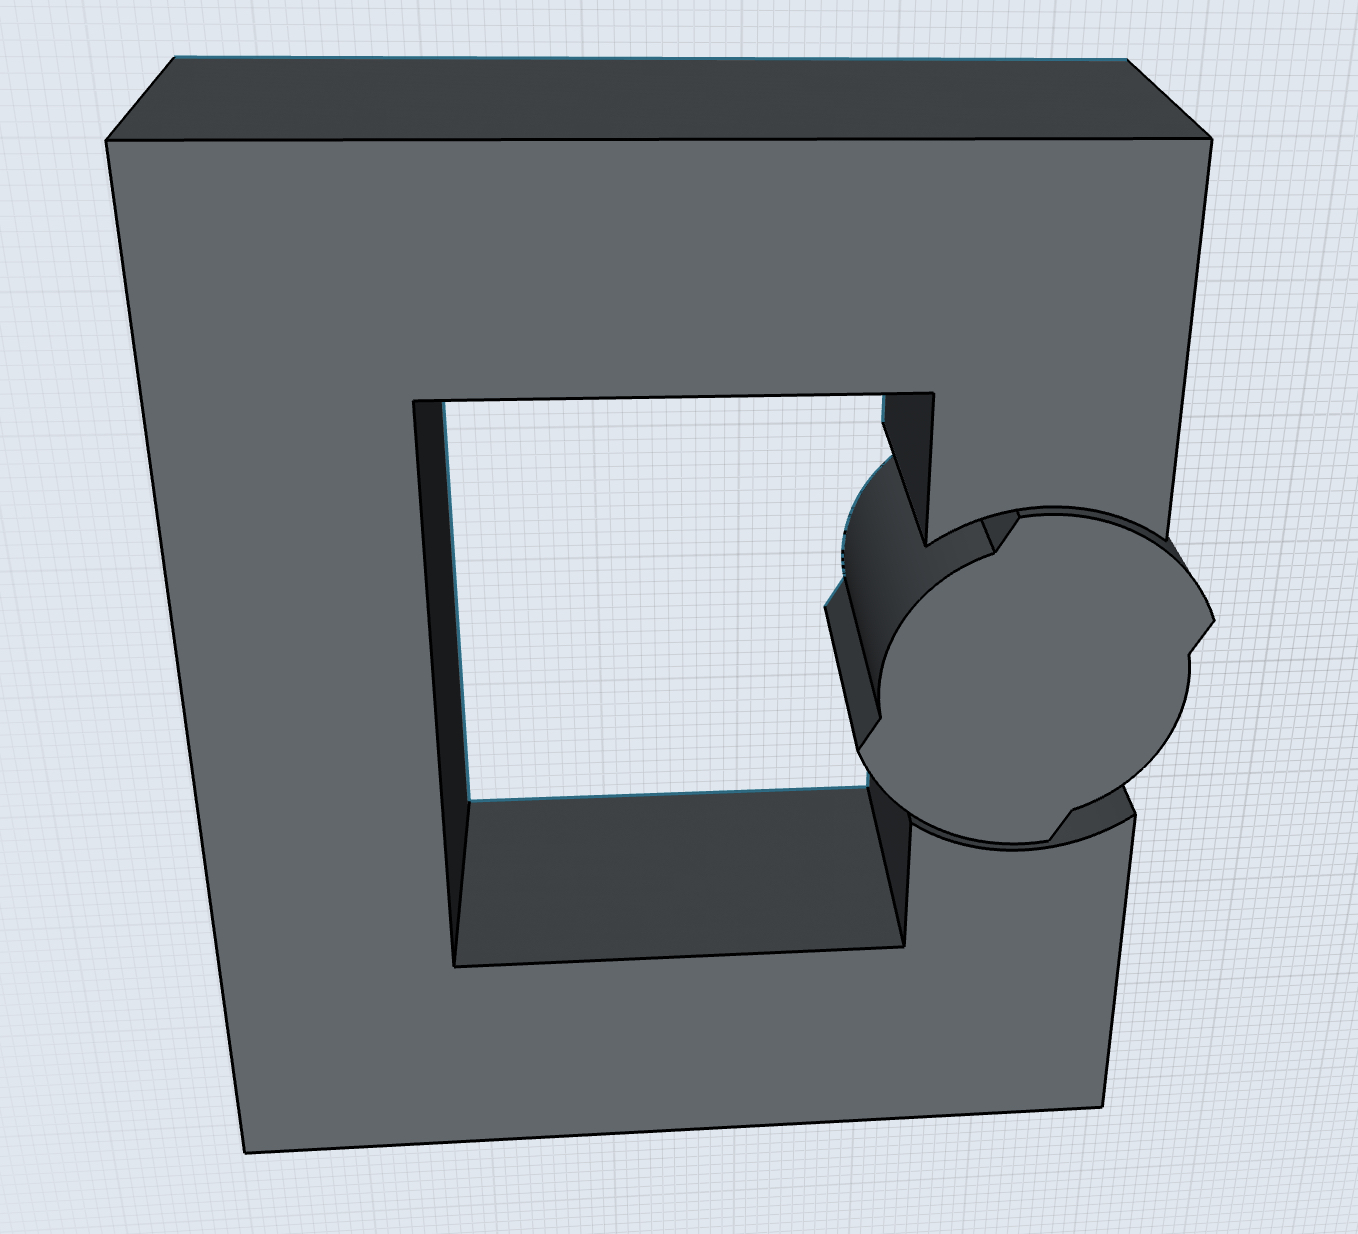
\includegraphics[width=\linewidth]{../core.jpeg}
    \caption{3-D view of the machine.}
    \label{fig:core3d}
  \end{subfigure}
  \hfill
  \begin{subfigure}{0.50\textwidth}
    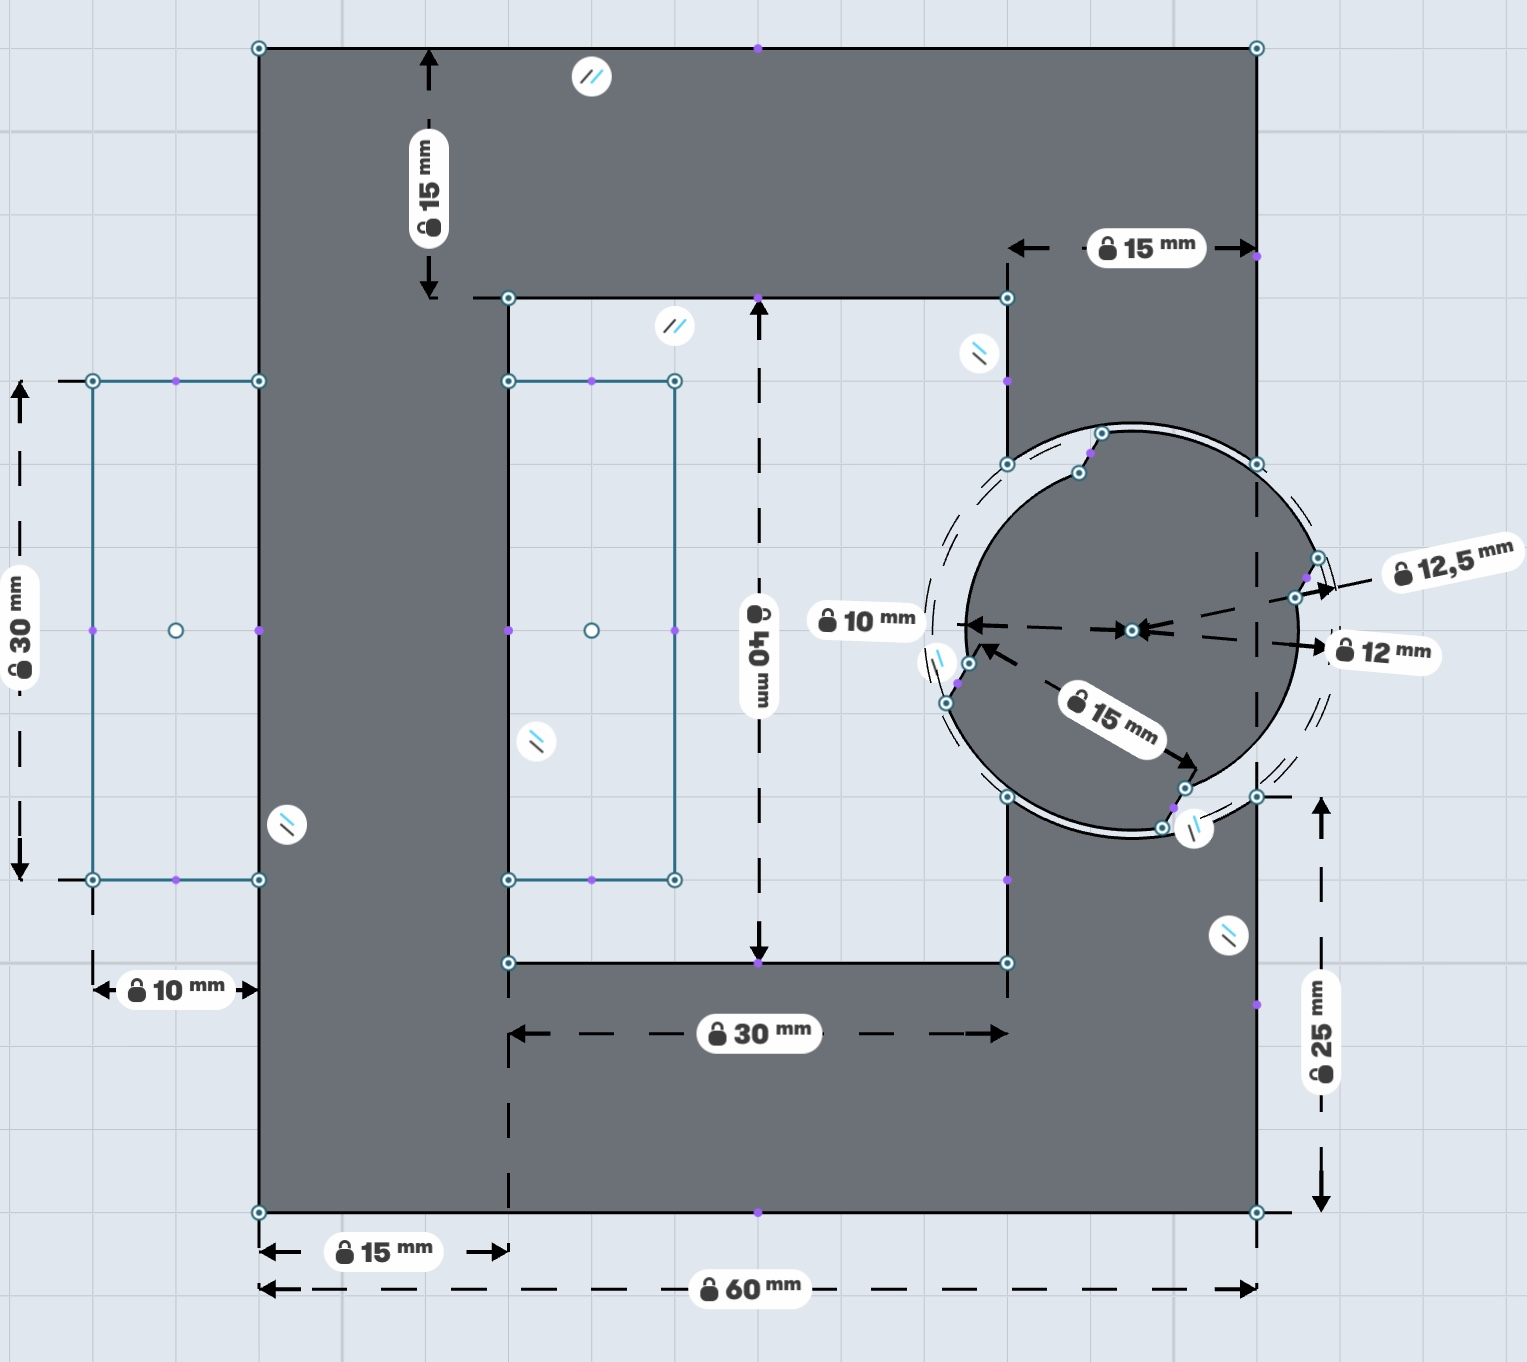
\includegraphics[width=\linewidth]{../dimensions.jpeg}
    \caption{2-D dimensioned drawing.}
    \label{fig:dimensions}
  \end{subfigure}
  \caption{Variable reluctance machine geometry.}
  \label{fig:geometry}
\end{figure}

\begin{table}[H]
  \centering
  \caption{Machine parameters.}
  \label{tab:params}
  \renewcommand{\arraystretch}{1.3}
  \begin{tabular}{|l|c|r|l|}
    \hline
    \textbf{Parameter}             & \textbf{Symbol} & \textbf{Value} & \textbf{Unit} \\
    \hline
    Number of turns                & $N$    & 300  & --  \\
    DC coil current                & $I$    & 2.5  & A   \\
    Air-gap clearance (each side)  & $g$    & 0.5  & mm  \\
    Core depth                     & $d$    & 25   & mm  \\
    Core / yoke width              & $w_c$  & 15   & mm  \\
    Stator inner window (width)    & $w_w$  & 30   & mm  \\
    Stator inner window (height)   & $h_w$  & 40   & mm  \\
    Rotor outer radius             & $R_r$  & 12.5 & mm  \\
    \hline
  \end{tabular}
\end{table}

\subsection{Assumptions}

To keep the analytical model tractable, the following assumptions are made:

\begin{enumerate}[label=\alph*)]
  \item The core is \textbf{infinitely permeable} ($\mu_r \to \infty$),
        so only the air-gap reluctance matters.
  \item There is \textbf{no fringing flux} -- the effective flux area
        equals the geometric core cross-section.
  \item The \textbf{inductance varies sinusoidally} with twice the
        mechanical angle, which is a standard approximation for a 2-pole
        machine.
  \item The system is \textbf{lossless} -- no eddy-current or hysteresis
        effects.
\end{enumerate}

\subsection{Core Geometry}

\textbf{Core cross-sectional area:}
\begin{equation}
  A_{\mathrm{core}} = w_c \times d = 15 \times 25 = 375\unit{mm^2}
  = 375 \times 10^{-6}\unit{m^2}
\end{equation}

\textbf{Mean magnetic path length} (centre-line of the stator):
\begin{align}
  \ell_{\mathrm{core}}
    &= 2(w_w + w_c) + 2(h_w + w_c) \notag \\
    &= 2(30+15) + 2(40+15) = 200\unit{mm} = 0.2\unit{m}
\end{align}

With the infinite-permeability assumption the core reluctance is zero,
so $\ell_{\mathrm{core}}$ plays no role in the inductance calculation
(it becomes relevant when finite permeability or saturation is
included in Section~\ref{sec:improve}).

\textbf{Air-gap lengths.} The flux crosses two gaps in series:

\begin{itemize}
  \item \emph{Aligned} ($\theta = 0^{\circ}$): both gaps equal the
        design clearance:
        \[
          \ell_{g,\min} = 2g = 2 \times 0.5 = 1\unit{mm}
        \]
  \item \emph{Unaligned} ($\theta = 90^{\circ}$): the rotor flat
        faces the pole tips, increasing each gap to $2.5\unit{mm}$:
        \[
          \ell_{g,\max} = 2 \times 2.5 = 5\unit{mm}
        \]
\end{itemize}

\subsection{Maximum and Minimum Inductance}

With an infinitely permeable core the reluctance is purely due to
the air gap:
\begin{equation}
  \mathcal{R} = \frac{\ell_g}{\mu_0 A_{\mathrm{core}}}
  \qquad \Rightarrow \qquad
  L = \frac{N^2}{\mathcal{R}} = \frac{N^2 \mu_0 A_{\mathrm{core}}}{\ell_g}
\end{equation}

\textbf{At the aligned position} ($\ell_g = \ell_{g,\min} = 1\unit{mm}$):
\begin{align}
  \mathcal{R}_{\min}
    &= \frac{1\times10^{-3}}{4\pi\times10^{-7}\times375\times10^{-6}}
     = 2.122\times10^{6}\unit{A/Wb} \\
  L_{\max}
    &= \frac{300^2}{2.122\times10^{6}} = 42.41\unit{mH}
\end{align}

\textbf{At the unaligned position} ($\ell_g = \ell_{g,\max} = 5\unit{mm}$):
\begin{align}
  \mathcal{R}_{\max}
    &= \frac{5\times10^{-3}}{4\pi\times10^{-7}\times375\times10^{-6}}
     = 10.61\times10^{6}\unit{A/Wb} \\
  L_{\min}
    &= \frac{300^2}{10.61\times10^{6}} = 8.48\unit{mH}
\end{align}

The results are summarised in Table~\ref{tab:LR}.

\begin{table}[H]
  \centering
  \caption{Reluctance and inductance at the two extreme positions.}
  \label{tab:LR}
  \renewcommand{\arraystretch}{1.3}
  \begin{tabular}{|l|c|c|c|}
    \hline
    \textbf{Position} & $\ell_g$ (mm) & $\mathcal{R}$ (MA/Wb) & $L$ (mH) \\
    \hline
    Aligned ($\theta = 0^{\circ}$)    & 1.0 & 2.122 & 42.41 \\
    Unaligned ($\theta = 90^{\circ}$) & 5.0 & 10.61 & 8.48  \\
    \hline
  \end{tabular}
\end{table}

\subsection{Inductance Variation $L(\theta)$}

Assuming a sinusoidal variation between $L_{\min}$ and $L_{\max}$:

\begin{equation}
  \boxed{L(\theta) = \frac{L_{\max}+L_{\min}}{2}
    + \frac{L_{\max}-L_{\min}}{2}\cos(2\theta)}
  \label{eq:Ltheta}
\end{equation}

This satisfies $L(0^{\circ}) = L_{\max}$ and $L(90^{\circ}) = L_{\min}$.
The factor $2\theta$ reflects the 2-pole symmetry: one full inductance
cycle every $180^{\circ}$ of mechanical rotation.

\subsection{Torque $T(\theta)$}

For constant current excitation the torque is the co-energy derivative:
\begin{equation}
  T(\theta) = \frac{1}{2}\,i^2\,\frac{dL}{d\theta}
  \label{eq:Tcoenergy}
\end{equation}

Differentiating Equation~(\ref{eq:Ltheta}):
\begin{equation}
  \frac{dL}{d\theta} = -(L_{\max}-L_{\min})\sin(2\theta)
\end{equation}

So the torque is:
\begin{equation}
  \boxed{T(\theta) = -\frac{i^2}{2}(L_{\max}-L_{\min})\sin(2\theta)}
  \label{eq:Ttheta}
\end{equation}

The peak torque amplitude at $I = 2.5\unit{A}$:
\begin{align}
  T_{\mathrm{peak}}
    &= \frac{I^2}{2}(L_{\max}-L_{\min}) \notag \\
    &= \frac{(2.5)^2}{2}\times(42.41-8.48)\times10^{-3}
     = 106.0\unit{mN\cdot m}
  \label{eq:Tpeak}
\end{align}

The average torque under constant DC is zero (positive and negative
halves cancel). The inductance and torque plots are shown in
Figure~\ref{fig:LT}.

\begin{figure}[H]
  \centering
  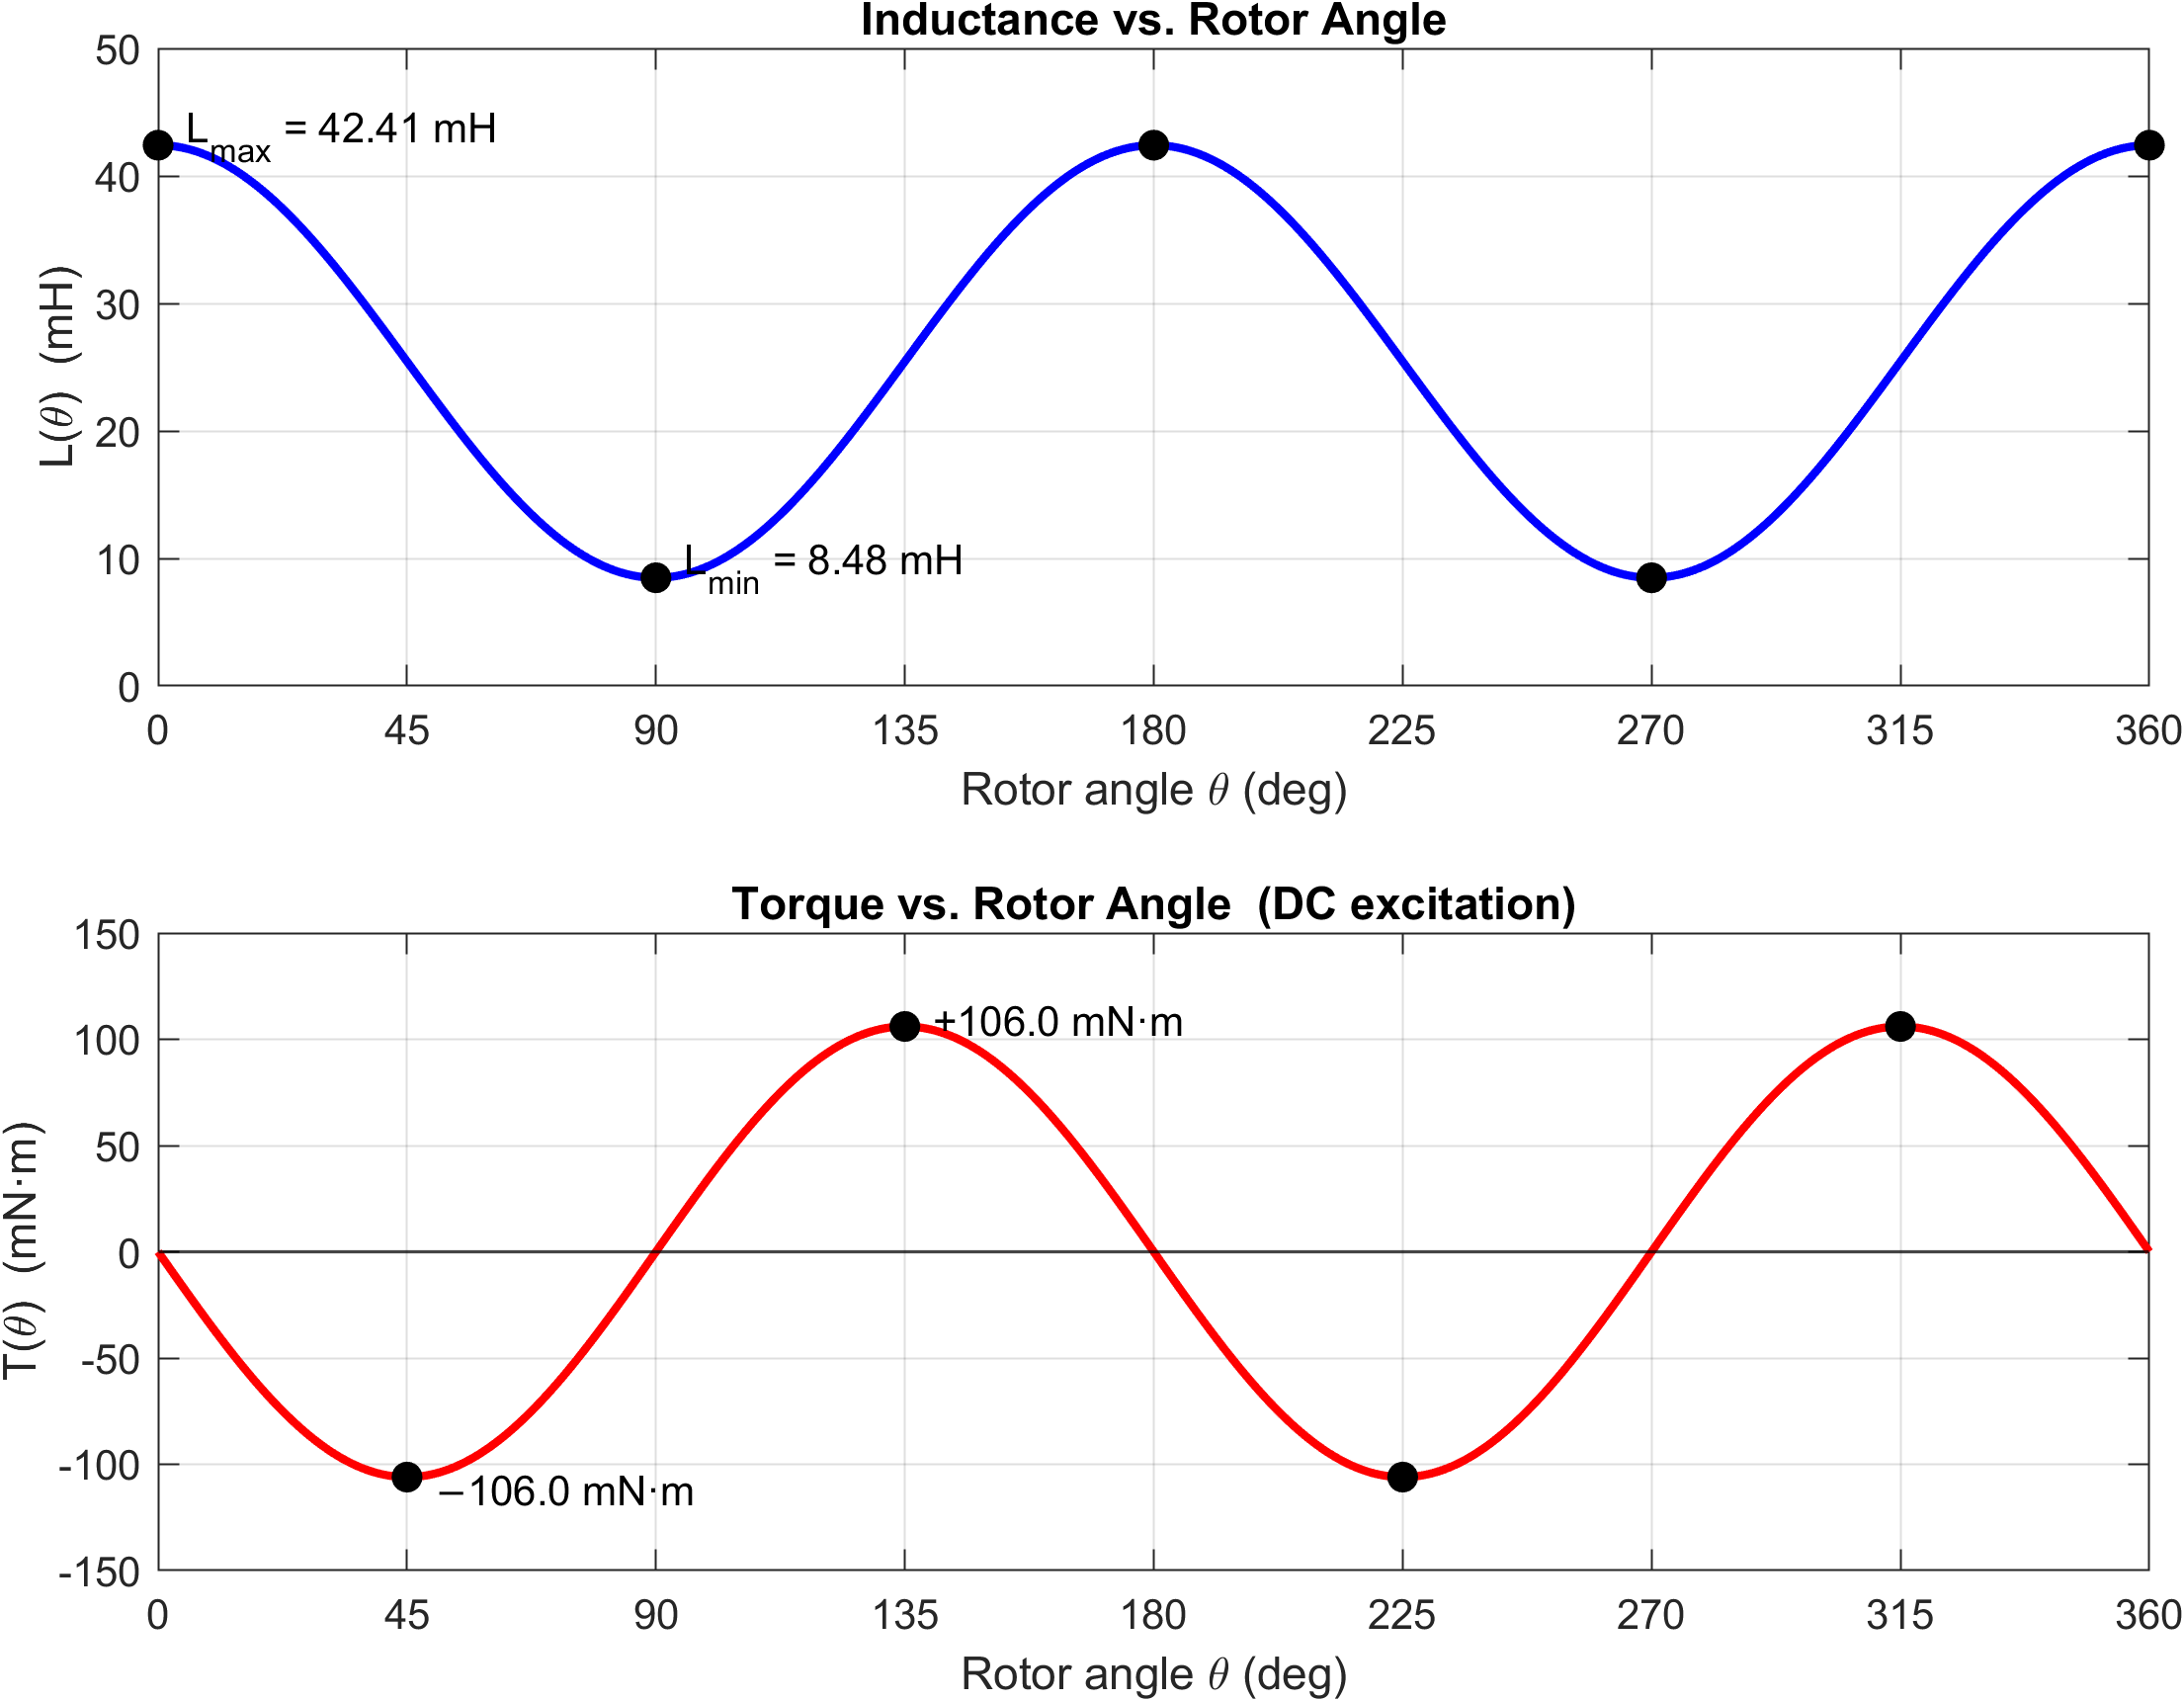
\includegraphics[width=0.95\textwidth]{../analytical_LT_plots.png}
  \caption{Inductance (top) and torque (bottom) vs.\ rotor angle,
           from the analytical model. $L$ ranges from $8.48\unit{mH}$
           to $42.41\unit{mH}$; peak torque is $\pm106\unit{mN\cdot m}$.}
  \label{fig:LT}
\end{figure}

\subsection{Improving the Model}
\label{sec:improve}

The main limitations of the model above and how to address them:

\begin{enumerate}
  \item \textbf{Finite core permeability.} Including the core
        reluctance $\mathcal{R}_{\mathrm{core}} =
        \ell_{\mathrm{core}}/(\mu_0\mu_r A_c)$ in series with the
        air-gap reluctance reduces $L_{\max}$ and changes the
        $L_{\max}/L_{\min}$ ratio.  For silicon steel
        ($\mu_r \approx 5000$) this effect is on the order of a few
        percent.

  \item \textbf{Magnetic saturation.} At high currents $\mu_r$ drops
        and $L$ becomes a function of both $\theta$ and $i$.
        The torque must then be computed from the full co-energy
        integral $T = \partial W'(\theta,i)/\partial\theta$.

  \item \textbf{Fringing flux.} The effective flux area at the gap
        edges is larger than $A_{\mathrm{core}}$.  A simple correction
        replaces $w_c$ and $d$ with $(w_c+\ell_g)$ and $(d+\ell_g)$,
        which increases both $L_{\max}$ and $L_{\min}$ (more so at the
        larger gap). A 2-D FEA captures this automatically.

  \item \textbf{Non-sinusoidal profile.} The actual inductance
        variation follows the change in overlapping pole-arc area with
        angle and is closer to a trapezoidal shape than a sinusoid.
        This can be captured analytically by integrating the air-gap
        permeance over the overlap area as a function of $\theta$.
\end{enumerate}

%% ============================================================
\section{Q2 -- FEA Modelling (Linear Materials)}

\textit{The 2D FEA simulation with linear material properties is
performed in FEMM.  Results will be added to this section.}

\subsection{Model Setup}
\begin{itemize}
  \item Software: FEMM 4.2 (2D magneto-static).
  \item Core: \textit{[material, linear $\mu_r$ = \ldots]}.
  \item Positions: $0^{\circ}$, $45^{\circ}$, $90^{\circ}$.
\end{itemize}

\subsection{Flux Density Plots}
\textit{[Insert flux-density vector plots for three positions.]}

\subsection{Inductance and Stored Energy}
\textit{[Insert results table for $\theta = 0^{\circ}$, $45^{\circ}$,
$90^{\circ}$.]}

\subsection{Torque vs.\ Angle -- Comparison with Analytical Model}
\textit{[Insert torque vs.\ angle plot comparing FEA ($\geq 10$
positions) with Equation~(\ref{eq:Ttheta}).]}

%% ============================================================
\section{Q3 -- FEA Modelling (Non-Linear Materials)}

\textit{Same as Q2 but with a non-linear (saturating) $B$--$H$ curve.}

\subsection{Material Properties}
\textit{[Describe the $B$--$H$ curve; include the plot in the Appendix.]}

\subsection{Flux Density Plots}
\textit{[Insert plots for three positions.]}

\subsection{Inductance and Stored Energy}
\textit{[Insert results table.]}

\subsection{Torque vs.\ Angle}
\textit{[Insert torque vs.\ angle plot.]}

\subsection{Discussion}
\textit{[Compare linear vs.\ non-linear FEA and analytical model.
Discuss saturation, fringing, and the validity of the sinusoidal
assumption.]}

%% ============================================================
\section{Q4 -- Control Method for Continuous Rotation}
\label{sec:control}

\subsection{The Problem}

With constant DC current the torque averages to zero over a full
rotation. For net unidirectional motion the current must be switched
on only when it produces positive torque.

\subsection{Switched Excitation}

From Equation~(\ref{eq:Ttheta}), torque is positive when
$\sin(2\theta) < 0$, i.e.\ when
$\theta \in (90^{\circ}, 180^{\circ}) \cup (270^{\circ}, 360^{\circ})$.
The strategy is simple: \textbf{energise the coil as the rotor moves
from unaligned toward aligned; switch off before the aligned position
to avoid negative torque on the return stroke.}

\subsection{Average Torque}

With ideal on/off switching (on at $90^{\circ}$, off at $180^{\circ}$):
\begin{align}
  T_{\mathrm{avg}}
    &= \frac{1}{\pi}\int_{90^{\circ}}^{180^{\circ}}
       \frac{I^2}{2}(L_{\max}-L_{\min})(-\sin 2\theta)\,d\theta
     = \frac{T_{\mathrm{peak}}}{\pi}
     \approx \frac{106.0}{\pi}
     \approx 33.8\unit{mN\cdot m}
\end{align}

This is about $31.8\%$ of the peak torque.

\subsection{Practical Considerations}

\begin{itemize}
  \item A position sensor (Hall effect or encoder) is needed to
        synchronise switching with rotor angle.
  \item The turn-on angle should be slightly before $90^{\circ}$ and
        the turn-off angle slightly before $180^{\circ}$ to compensate
        for the finite current rise and fall times.
  \item A PWM current controller keeps the current constant during the
        on-interval for repeatable torque.
\end{itemize}

%% ============================================================
\section{Conclusion}

The analytical model predicts an inductance variation from
$L_{\min} = 8.48\unit{mH}$ to $L_{\max} = 42.41\unit{mH}$, with a
peak torque of $106\unit{mN\cdot m}$ under $2.5\unit{A}$ DC.
Constant DC excitation produces zero average torque; switching the
current on during the unaligned-to-aligned transition raises the
average to approximately $33.8\unit{mN\cdot m}$.
FEA results (linear and non-linear) will be added to refine these
estimates and quantify the effects of fringing and saturation.

%% ============================================================
\appendix
\section{MATLAB Code}

\lstinputlisting[style=matlab,
  caption={Analytical inductance and torque script
           (\texttt{analytical\_model.m}).}]{../analytical_model.m}

\section{Material Properties}
\textit{[Insert $B$--$H$ curve data for the steel used in Q2/Q3.]}

\end{document}
